\section{Mining Next Generation}
\label{sect:mining}

Traditionally blocks in a blockchain refer to an ordered list of
transactions combined with a cryptographic hash of the previous block
\cite{whatisablockchain,raikwar2019sok}. A hash function maps a
binary of any size to a fixed size binary. The aeternity blockchain
uses the 32 byte Blake2b hash \cite{aumasson2013blake2}. Cryptographic
hashes are collision resistant, making it very unlikely that two binaries
result in the same 32 bytes hash. It is also cryptographically hard
to find a binary that results in a given hash.

The sequence of cryptographic hashes in a blockchain avoid
that a transaction on the chain is tampered with. If a transaction
changes with even one bit, the hash of the block will change and the
next block will point to a non-existing hash. An attacker that
modifies a transaction in a block will have to modify all consecutive
blocks. If the hash is then also used to solve a cryptographic puzzle,
that consumes time to solve, but is easy to verify, then each hash
modification consumes time and is therefore increasingly costly the
more hashes have to be changed.

Many blockchains provide such a Proof-of-Work (PoW) puzzle and the agent
trying to solve the puzzle is called a \textit{miner} (cf. \ \cite{wang2018survey} for a more
refined view).  In Aeternity the \textit{Cuckoo}
algorithm is used as cryptographic puzzle \cite{Tromp2015CuckooCA}. This
algorithm was designed to be memory bound, meaning that large memories
have an advantage over fast computing with little memory. This makes
the algorithm less energy consuming than algorithms that are
computation bound.

\subsection{Mining to resolve solution conflicts}

In a distributed system, like the aeternity blockchain, there are many
computers (nodes) that together build the blockchain. Each of these nodes
can receive user signed transactions. Each of them will try to build a
block of these transactions and put it on the chain. Adding the next
block to the chain is rewarded directly with tokens. As soon as they
have created such a block and solved the corresponding cryptographic
puzzle, they gossip it to the other nodes in the network. This results
in the evident challenge for each node to decide  which of the blocks
it receives is the one that is the next block for the chain. There
must be a commonly agreed best block.

This challenge is addressed in two ways, on the one hand it is made far
less likely that a node receives two competing blocks by adding the previously
mentioned cryptographic puzzle. If a solution can on average only be found
every 3 minutes (in Aeternity), then it is unlikely that two blocks are
mined at almost the same instance.

Moreover, if the solution to the
cryptographic problem is easy to verify, faking a solution and spamming the
node with bad blocks is also much more difficult
\cite{miningagainstspamming}.

\subsubsection{Cuckoo PoW}

The Cuckoo algorithm has an adaptable complexity. Simply put it
searches for cycles of specific length in a graph with a given length
for the nodes. In the aeternity blockchain the length of the cycle is 42 and the size
of the nodes is 30 bits. By also demanding a number of
leading zeros in the solution (the difficulty), a solution can dynamically be made
more or less easy to find. It is cryptographically unlikely that two
solutions are exactly the same, since two miners will not create the
same block (the block contains the address of the miner receiving the
mining reward, as well as a 64-bit nonce that is selected at random to
solve the PoW problem).

The adaptable complexity allows us to keep the average time it takes
to find a solution around 3 minutes, independent of how many miners
are trying to solve it. By measuring the average creation speed of the
last 17 blocks, we can compute whether more or less miners are active and adjust
the difficulty accordingly. The difficulty is deterministically
computed and part of the block. In addition a timestamp is provided in
the block. This timestamp is unreliable, since the nodes have no
synchronized clocks. However, the timestamp may not precede the
timestamp of a previous block. A malicious miner that presents a
block with difficulty that diverts from the target specified in the
previous block will have its block refused by the chain. Likewise, if
a miner presents the wrong target difficulty for the next block, this
block will be discarded.

\subsubsection{Forks}

Due to network latency, not all nodes are guaranteed to receive
all blocks at the same time.  Therefore, a situation may occur in
which part of the network first receives block $A$ and then block $B$,
whereas the other nodes receives them in order first $B$ and then
$A$. The situation in which this happens and two nodes have different
top blocks, is called a \textit{fork}. In fact, due to for example a network
split in which several nodes are isolated for a while, forks can be
longer than just one block.

If blocks are gossiped to a node, then the total
difficulty of the fork determines
which branch to select. So in the unlikely case that a fork is
created, there is a consensus over how to restore the branch with
highest difficulty.

A different kind of fork is created when one part of the nodes does
not accept a block that the other nodes do accept as a valid block. This
can be caused by having the nodes run different versions of the
software that have an incompatibility. These forks are not
automatically restored and are referred to as \textit{hard forks}.

\subsection{Scaling transaction confirmations}

A user that submits a transaction has to wait for the transaction to
be part of a block, before it can be considered a valid
transaction. In fact, due to the previously described fork possibility due
to network latency, one may have to see the transaction in a block
followed by two more blocks to be reasonably sure that the chain will
perpetually keep that transaction. The longer one waits, the more certainty.

A transaction may be invalid for several reasons and even valid
transactions may not always be accepted on chain. There might be other transactions in
flight that have impact on the validity of the posted
transaction. Since one cannot assume in which order miners put
the  transactions in a block, just looking at a pool of not yet
included transactions gives very little certainty for the receiver of
funds associated with that transaction \cite{karame2012double}.

In many applications a quick temporary confirmation with little
definite certainty would be an advantage over more certainty, but
waiting longer. A commonly used example is a coffee shop. The price of
a cup of coffee may make a shop owner willing to serve the coffee if an
early indication gives some guarantee that the transaction is at least
acceptable for some miner.

\subsubsection{Key-blocks and micro-blocks}

In Aeternity we use bitcoin NG \cite{Eyal:2016:BSB:2930611.2930615} to
address this problem. Bitcoin NG boils down to collectively accepting the miner of a
block, called a \textit{key-block} in this context, as the
\textit{leader}. This leader is allowed to periodically publish micro-blocks with
transactions, until the next miner is elected the leader by presenting a
new key-block. Only for key-blocks a cryptographic puzzle needs to be
solved, thus there is very little cost in publishing micro-blocks with
transactions. In Aeternity the leader is allowed to publish a
micro-block including transactions every 3 seconds. This means that
users can see an accepted transaction much faster than after 3
minutes. This is just a preliminary confirmation, but one that is
stronger than having a transaction arrive in the transaction pool.

The derived 3 seconds per micro-block make sure that less powerful
computation units can stay synchronized with the chain. The
transactions in each micro-block need to be verified, which means
computation time (verification of cryptographic signatures, running
contracts, lookup data in previous blocks). In order to have a
reasonably predictable computation task, each micro-block is limited to
a maximum of 6 million gas and on the aeternity blockchain all
transactions are associated with a gas cost. Even on a low-end computer that should
not take more than a second to execute. The network latency and a good margin
are accommodated in the other two seconds.

Terminology wise, the height of the chain is determined by the
key-blocks, incrementing the height by one for each new key-block put
on the chain. Micro-blocks follow a key-block and are on the same
height. A key-block and the micro-blocks on the same height are
together called a \textit{generation}. Since key-blocks do not contain
transactions, but the micro-blocks do, one could conceptually see the
generations as the blocks in the more traditional blockchain view.

The key-blocks should contain the hash of the previous micro-block as
well as the hash of the previous key-block. This means that miners
preferably update their crypto puzzle as soon as a micro-block
arrives, because, if a miner is slow in updating the puzzle and finds a solution for an earlier
micro-block, then all following micro-blocks are discarded. This is
called a micro-fork, a key-block is mined on a micro-block that is not
the last micro-block produced. Compared to forks on key-blocks,
micro-forks occur relatively often. The
transactions of the produced and discarded micro-blocks are put back in the
transaction pool and taken care of by the next leader. Since they have
been seen in a micro-block before, they will very likely be valid in
future micro-block as well. In Aeternity there is an incentive to mine
on top of the newest micro-block, because the fees are divided by rewarding 40\%
to the leader producing a micro block and 60\% to the miner mining the key-block after that
micro-block\footnote{Note that if miners
  were to only mine key-blocks, there would be no transactions on the
  chain at all.}.

\begin{figure}
   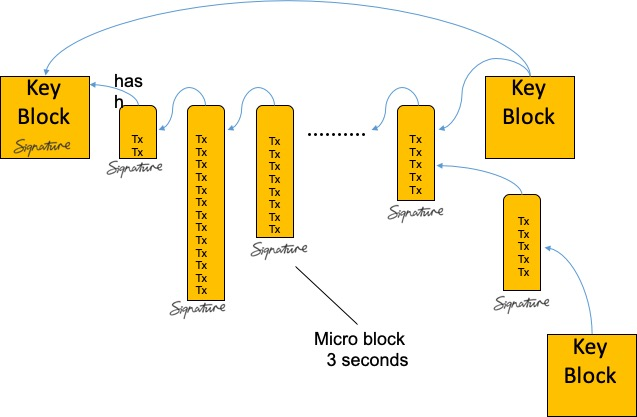
\includegraphics[scale=0.5]{keymicro.jpg}
  \caption{Micro forks}
\end{figure}

\subsubsection{Fraudulent leaders}

Only the leader is allowed to produce micro-blocks. Each key-block
includes the  public key of the next leader and consecutive micro-blocks are only valid
if signed with private key associated with it.. This protects against third parties trying
to post micro-blocks and all micro-blocks should form a well-defined
sequence.

A malicious leader, however, could construct forks in a generation of micro
blocks, either by forking directly from the key-block, or by forking
on a micro-block. This could be done to disrupt the network or to
perform double spend attacks. A malicious miner could also try to
produce more micro-blocks than entitled to by fiddling with the
micro-block creation timestamp.

In order to mitigate the risk of a leader forking its own sequence,
there is a mechanism in place to detect and report this by submitting
a Proof-of-Fraud. This is typically submitted in the next
generation. The leader is punished by not receiving a block reward and
in order to make that possible, block rewards are not immediately paid out but kept for
the duration of 180 blocks.

\subsubsection{Divide and conquer}

Each transaction is a binary of a certain size. Internally both size
and computation are expressed in gas and there is a maximum amount of
gas per micro-block that allows for maximally 300KB per micro-block.
Thus, an additional advantage of the introduction of micro-blocks is that
instead of a huge block with 180,000 transactions in 3 minutes, we can create 60
reasonably sized micro blocks of maximally 300 KB  in the same 3
minutes. This has several advantages for network latency and
smaller blocks are easier and faster to gossip through the
network. Moreover, if it takes longer to compute the next key-block we
are not bound to a maximum block size, because we generate new
micro-blocks as long as no key-block has been found. Yet another
scaling advantage of NG.
